%% LyX 1.6.7 created this file.  For more info, see http://www.lyx.org/.
%% Do not edit unless you really know what you are doing.
\documentclass[english]{scrartcl}
\renewcommand{\familydefault}{\sfdefault}
\usepackage[T1]{fontenc}
\usepackage[latin9]{inputenc}
\usepackage[a4paper]{geometry}
\geometry{verbose,tmargin=2cm,bmargin=3cm}
\setlength{\parskip}{\medskipamount}
\setlength{\parindent}{0pt}
\usepackage{babel}

\usepackage{array}
\usepackage{graphicx}
\usepackage[unicode=true, pdfusetitle,
 bookmarks=true,bookmarksnumbered=false,bookmarksopen=false,
 breaklinks=false,pdfborder={0 0 1},backref=false,colorlinks=false]
 {hyperref}

\DeclareGraphicsExtensions{.png,.jpg}

\makeatletter

%%%%%%%%%%%%%%%%%%%%%%%%%%%%%% LyX specific LaTeX commands.
%% Because html converters don't know tabularnewline
\providecommand{\tabularnewline}{\\}

%%%%%%%%%%%%%%%%%%%%%%%%%%%%%% User specified LaTeX commands.
\usepackage{color}
\usepackage{colortbl}

% Different font in captions
\newcommand{\captionfonts}{\small}
\makeatletter  % Allow the use of @ in command names
\long\def\@makecaption#1#2{%  
  \vskip\abovecaptionskip  
  \sbox\@tempboxa{{\captionfonts #1: #2}}%
  \ifdim \wd\@tempboxa >\hsize    
{\captionfonts #1: #2\par}  
  \else    
\hbox to\hsize{\hfil\box\@tempboxa\hfil}%
  \fi  
  \vskip\belowcaptionskip}
\makeatother   % Cancel the effect of \makeatletter

% Some default colors
\definecolor{red}{rgb}{1,0,0}
\definecolor{green}{rgb}{0,1,0}
\definecolor{blue}{rgb}{0,0,1}
\definecolor{lightgray}{gray}{0.8}
\definecolor{lightergray}{gray}{0.93}

\makeatother

\begin{document}

\title{SDMVIS Manual}


\date{Version 0.3 (2011-10-05)}


\author{Max Hermann{\normalsize }%
\thanks{\texttt{\protect\href{mailto:hermann@cs.uni-bonn.de}{hermann@cs.uni-bonn.de}}%
}}
\maketitle
\begin{abstract}
SDMVIS is a visual analysis software to explore statistical deformation
models (SDM) of volumetric organisms. Interactive exploration is facilitated
by integrating two kinds of expert knowledge: taxonomical or other
classifications of the datasets as well as knowledge about relevant
structures and parts of the shape. Given a classification into two
groups the corresponding dominant shape differences between the groups
(a so-called trait) can be computed and visualized in a dynamic fashion.
Based on a selected region of interest (ROI) a new weighted SDM can
be derived whose principal modes of shape variability are again accessible
in a dynamic visualization.
\end{abstract}
\tableofcontents{}

\pagebreak{}


\section{Overview\label{sec:Overview}}

%
\begin{figure}
\noindent \begin{centering}
\label{fig:pipeline}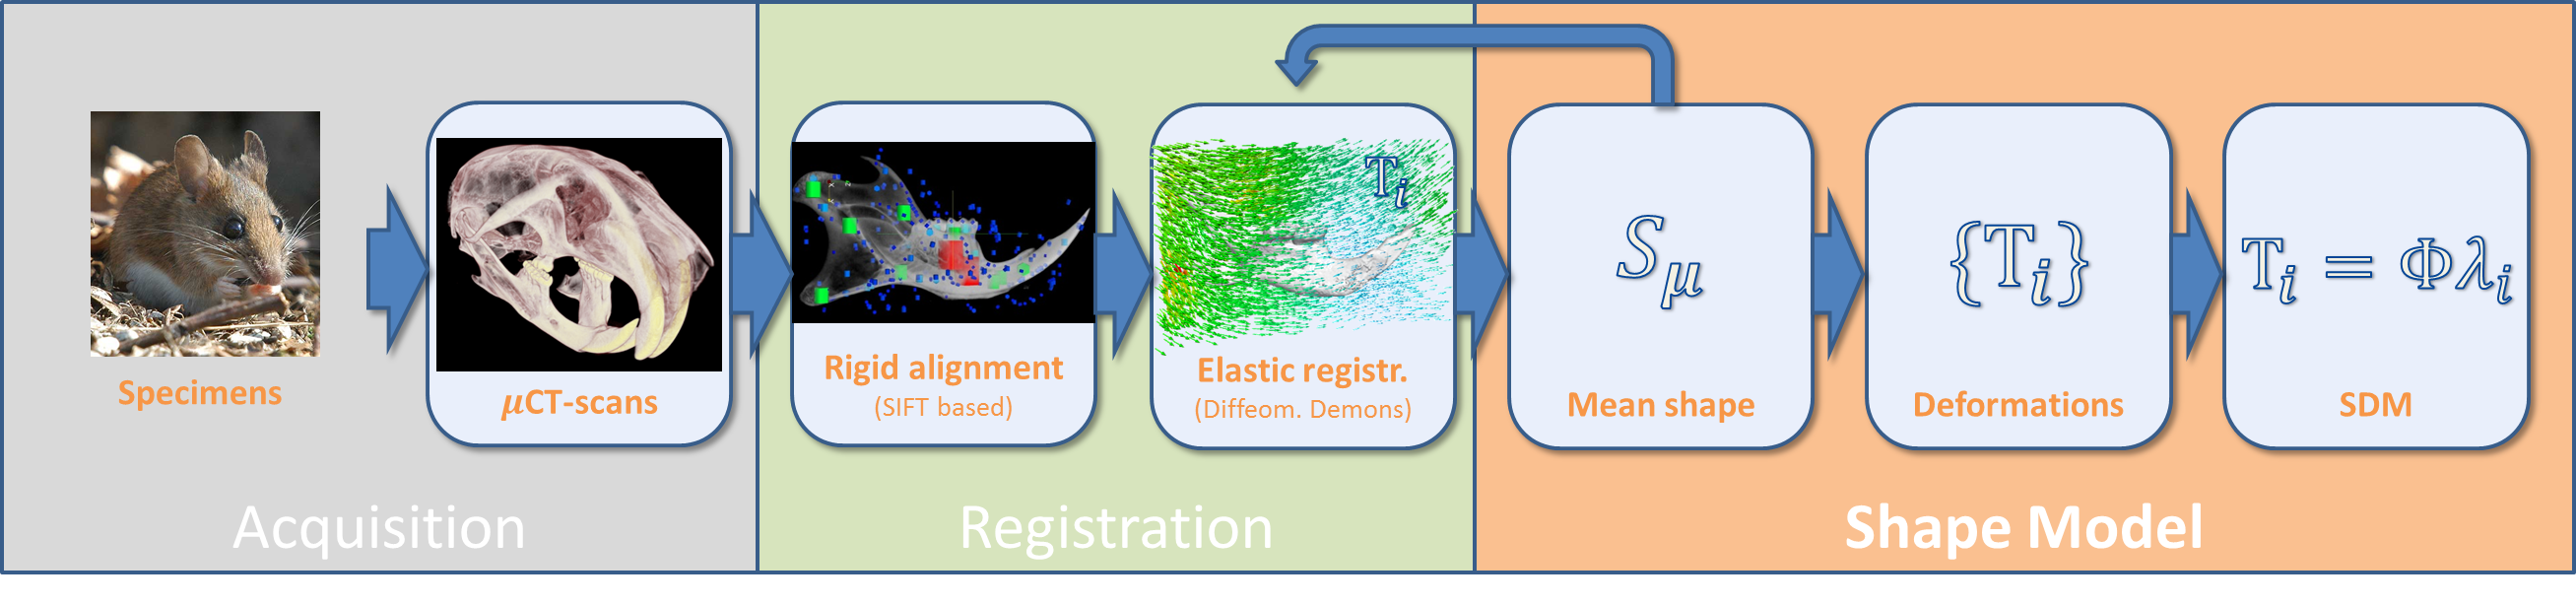
\includegraphics[width=1\textwidth]{images/pipeline}
\par\end{centering}

\caption{Processing pipeline from acquisition to shape model. SDMVIS is a tool
to explore a given shape model and derive new (sub-)models from it.
It also provides visualizations to assess registration quality.}

\end{figure}


%
\begin{figure}
\noindent \begin{centering}
\label{fig:gui}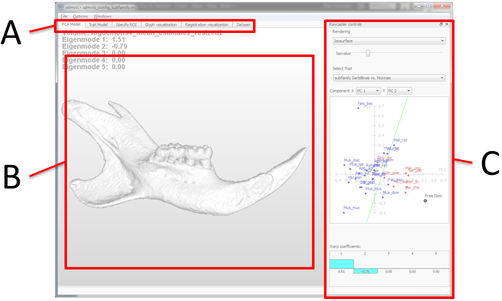
\includegraphics[width=0.8\textwidth]{screenshots/labels}
\par\end{centering}

\caption{SDMVIS user inteface overview: \textbf{(A)} Tab bar with available
visual analysis tasks which can be activated by clicking on the corresponding
tab entry. \textbf{(B)} Visualization of the active task. \textbf{(C)}
Control widget with options and controls for the active task.}

\end{figure}


SDMVIS assumes as input an already registered subset of your data,
see Figure~\ref{fig:pipeline}. For now an initial shape model has
also to be provided (which will hopefully soon be obsolete). The user
interface is designed task-oriented with respect to the following
visual analysis tasks:
\begin{itemize}
\item Investigate PCA model \texttt{\textbf{{[}PCA Model{]}}}
\item Investigate and/or compute trait model \texttt{\textbf{{[}Trait Model{]}}}
\item Spefiy a region of interest and compute a new PCA model \texttt{\textbf{{[}Specify
ROI{]}}}
\item Assess shape variability of an eigenwarp or trait in a static visualization
\texttt{\textbf{{[}Glyph visualization{]}}}
\item Assess registration quality visually \texttt{\textbf{{[}Registration
visualization{]}}}
\item Prepare results in a table e.g. for exporting to Excel \texttt{\textbf{{[}Dataset{]}}}
\end{itemize}
In braces the shorthand term for the specific task respectively mode
in SDMVIS is given. Only one mode can be active at a given time. The
user interface provides a tab-bar to switch between the different
modes. Each mode has its own controls and visualization as indicated
in Figure~\ref{fig:gui}.


\section{Data Management\label{sec:Data-Management}}

The data management concept is not finished yet. We currently rely
on configuration files which represent a specific analysis session
in SDMVIS, see also Table~\ref{tab:analysis_items}. To discern different
analyses an identifying keyword has to be specified by the user for
each analysis.

The current data management approach can be summarized as follows:
\begin{itemize}
\item Data files follow a specific naming convention.
\item Relevant files of a \emph{specific analysis} are stored in a single
directory.
\item A single \emph{configuration file} holds the needed filenames and
additional parameters of a specific analysis (see Table~\ref{tab:analysis_items}).
\item SDMVIS \emph{automatically} creates configuration files and the needed
directory structure for trait and/or ROI analyses.
\item For now, each analysis is identified by a user specified line of text
or a \emph{keyword}.
\end{itemize}
By performing a ROI selection a new SDM is derived for which a new
analysis with SDMVIS has to be performed. Thus SDMVIS automatically
creates a new configuration file which is loaded immediately after
creation. All relevant data files are stored in a sub-directory of
the original analysis configuration file. The new sub-directory is
named according to the new keyword specified for the ROI analysis.

Computing a new trait does not change the current SDM and the current
configuration file is simply updated. The newly created trait files
are stored in a sub-directory named according to the keyword of the
current analysis.

The datasets and mean estimate as well as all eigen- and traitwarps
are stored as Metaimage MHD files. These can be loaded and displayed
by most Visualization Software Packages like for example ParaView.

%
\begin{table}
\noindent \centering{}\label{tab:analysis_items}\begin{tabular}{|l|>{\raggedright}p{0.5\textwidth}|>{\raggedright}p{0.3\textwidth}|}
\hline 
\emph{Item} & \emph{Description} & \emph{Storage}\tabularnewline
\hline
\hline 
\rowcolor{lightergray}list of names & names of the analysed datasets & in configuration file\tabularnewline
\hline 
mean estimate & estimate of a mean shape or a reference dataset & .MHD volume\tabularnewline
\hline 
\rowcolor{lightergray}warpfields & warpfields describe the deformation of the mean to a specific dataset & single huge .MAT matrix\tabularnewline
\hline 
eigenwarps & high-dimensional PCA eigenvectors & single huge .MAT matrix\tabularnewline
\hline 
\rowcolor{lightergray}PCA model & low-dimensional scatter matrix, eigenvectors, eigenvalues & in configuration file\tabularnewline
\hline 
traits and traitwarps & a single trait is described in an custom configuration file & custom .TWF file\tabularnewline
\cline{2-3} 
\emph{(optional)} & low-dimensional trait vector & small .MAT vector\tabularnewline
\cline{2-3} 
 & high-dimensional traitwarp & .MHD volume\tabularnewline
\hline
\rowcolor{lightergray}ROI \emph{(optional)} & user selected region of interest (new specific analysis) & in configuration file\tabularnewline
\hline
\end{tabular}\caption{Items of a specific analysis}

\end{table}


\newpage{}


\section{Visualizations\label{sec:Visualizations}}


\subsection{PCA Scatterplots and Diagrams}

\noindent \begin{center}
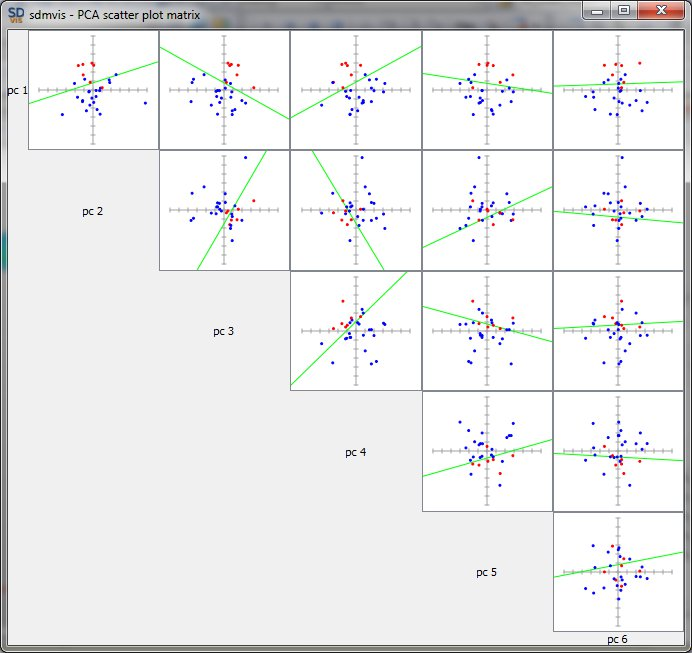
\includegraphics[height=6cm]{screenshots/scatterplotmatrix}
\par\end{center}
\begin{itemize}
\item groups are colored blue and red (if classification is available)
\item trait separating hyperplane is shown in green (if available)
\item in \texttt{{[}Trait Model{]}} view:

\begin{itemize}
\item single items may be selected by clicking on them
\item right click in diagram area opens context menu with further options
\item {}``Free Item'' mode provides dynamic visualization
\end{itemize}
\end{itemize}

\subsection{Dynamic Visualization of Deformation Fields}

\texttt{{[}PCA Model{]}} \texttt{{[}Trait Model{]}}

\noindent \begin{center}
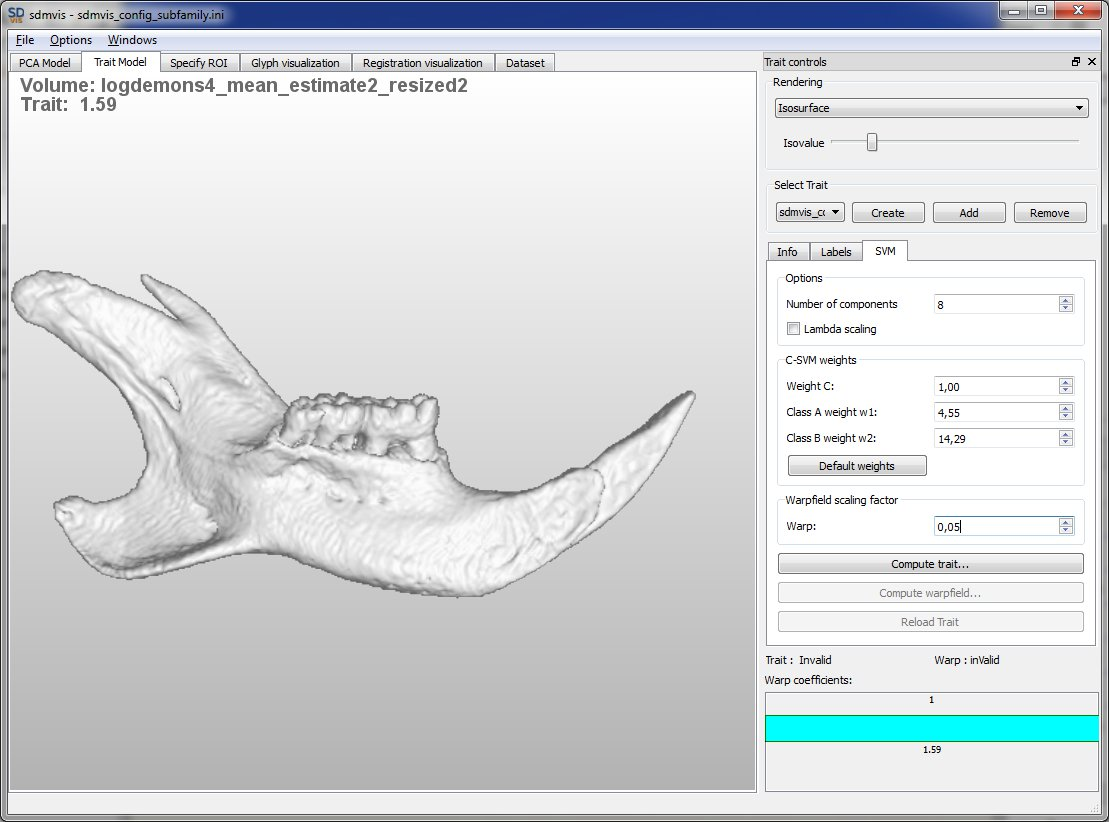
\includegraphics[height=6cm]{screenshots/sdmvis_traitmodel}
\par\end{center}
\begin{itemize}
\item warp coefficient(s) can be adjusted by manipulating the bar plot to
the lower right of the control widget
\item in \texttt{{[}PCA Model{]}} one can alternatively use the {}``Free
Item'' mode of the PCA plot (right click on the PCA diagram to activate
the context menu from which the Free Item mode can be set)
\item in \texttt{{[}Trait Model{]}} the warp scaling parameter has to be
adjusted manually
\end{itemize}

\subsection{Static Glyph Visualization of Deformation Fields}

\texttt{{[}Glyph visualization{]}}

\noindent \begin{center}
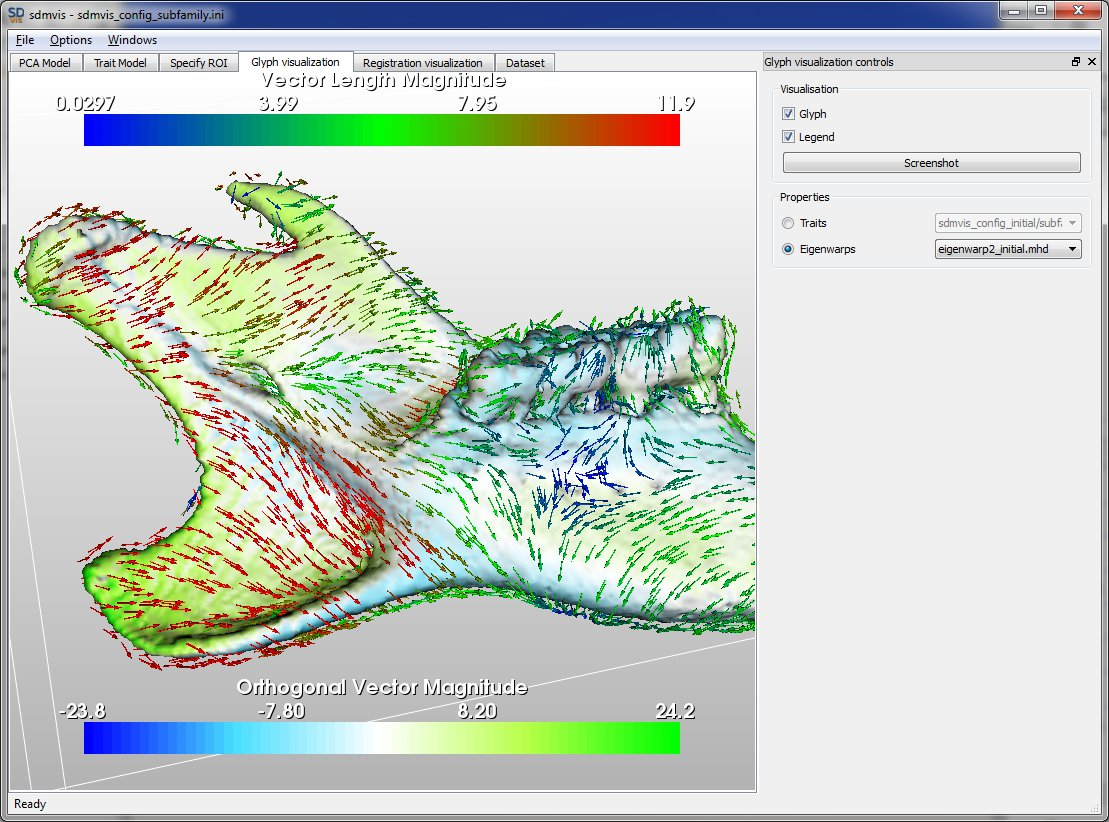
\includegraphics[height=6cm]{screenshots/sdmvis_glyphs}
\par\end{center}
\begin{itemize}
\item first, select in the control widget which trait or eigenwarp you want
to be visualized
\item color coding of the surface indicates growth/shrinking of the shape
\item glyph vectors represent tangential shift on the shape
\end{itemize}

\subsection{Comparative Visualization to assess Registration Quality}

\texttt{{[}Registration visualization{]}}

\noindent \begin{center}
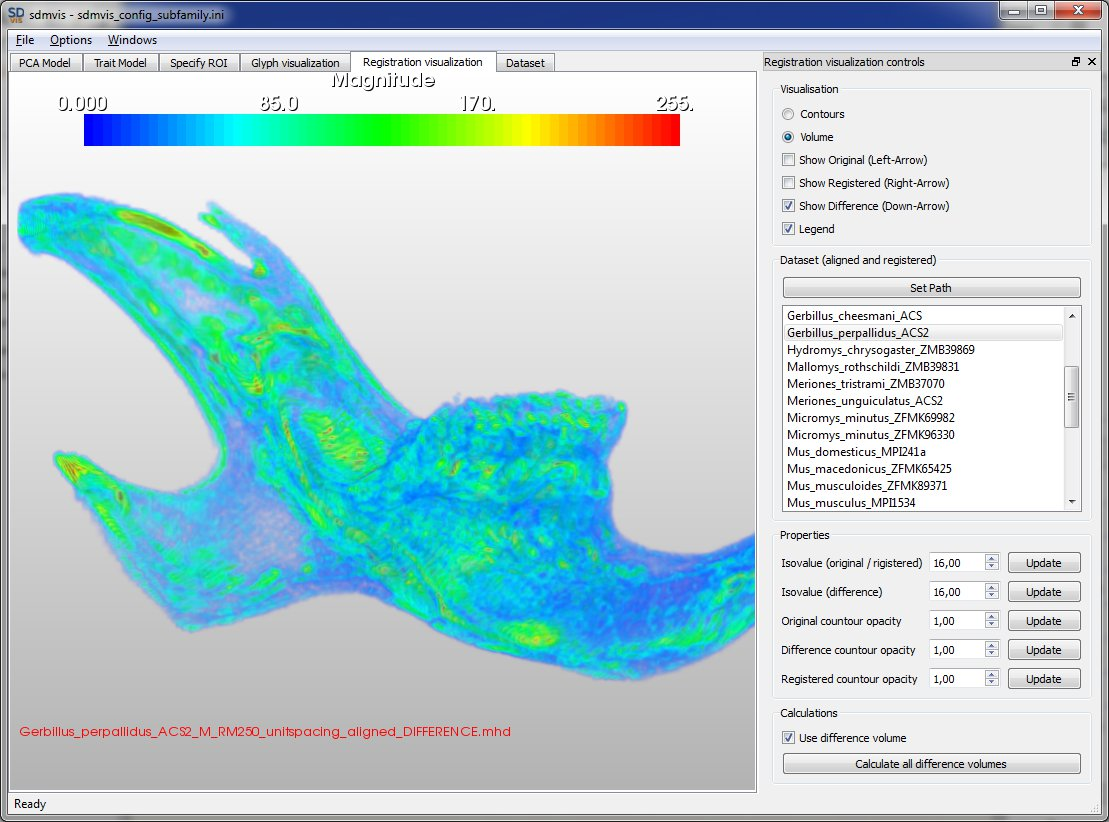
\includegraphics[height=6cm]{screenshots/sdmvis_regquality}
\par\end{center}
\begin{itemize}
\item needs aligned and registered datasets in a specific directory which
has to be selected via {}``Set Path'' in the control widget
\item can show the aligned original dataset in comparison to the deformed
mean estimate (which should match the original as closely as possible
for a faithfull investigation)
\item supports contour rendering of the surface as well as volume rendering
(in rainbow colors)
\item can compute and visualize the difference between the aligned and the
registered volume (as shown on the screenshot); this maybe a usefull
visualization to estimate the registration quality of specific areas
\end{itemize}

\subsection{Statistical Deformation Model Quality (not available yet)}

\newpage{}


\section{Analysis Tasks\label{sec:Analysis-Tasks}}


\subsection{PCA Model}

\texttt{{[}PCA Model{]}}

\noindent \begin{center}
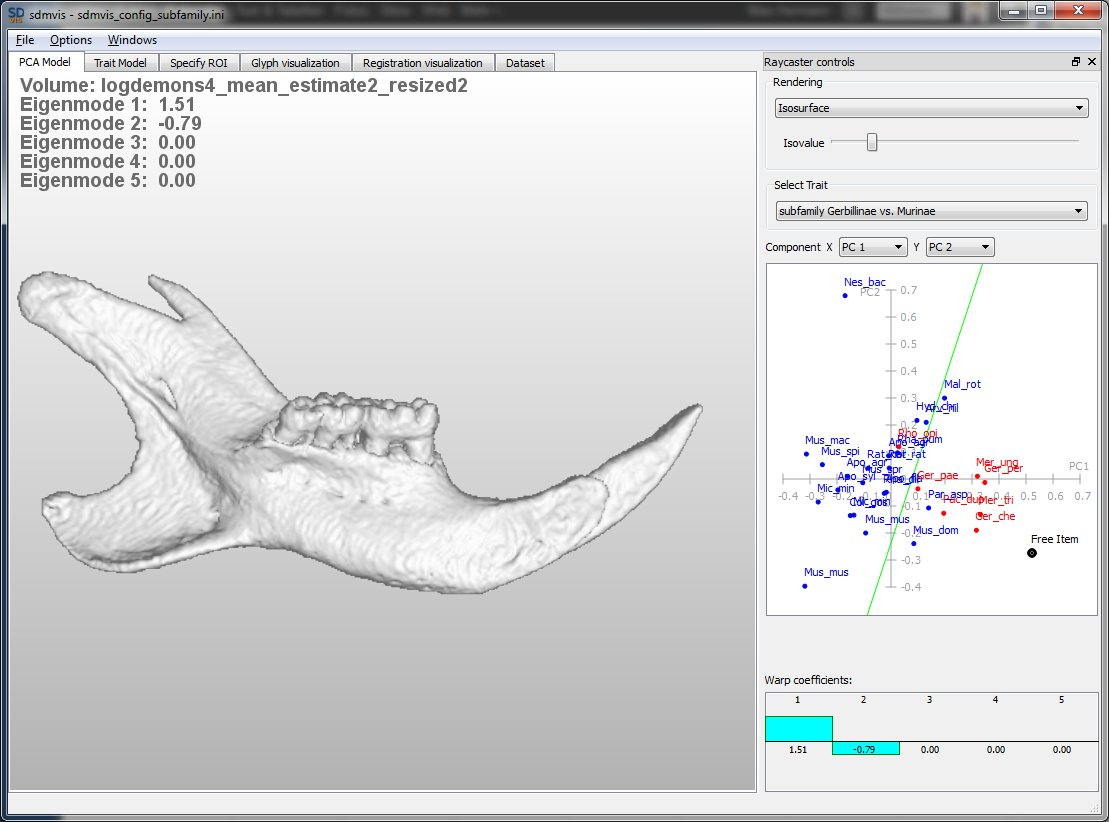
\includegraphics[height=6cm]{screenshots/sdmvis_pcamodel}
\par\end{center}


\subsection{Classification Trait Vector}

\texttt{{[}Trait Model{]}}

\noindent \begin{center}
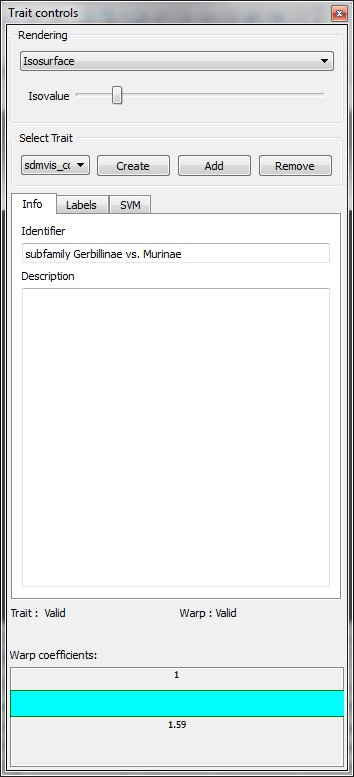
\includegraphics[width=0.2\textwidth]{screenshots/trait-ctrl-1}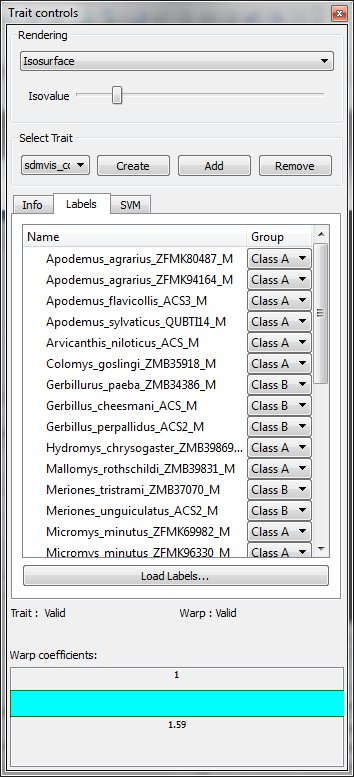
\includegraphics[width=0.2\textwidth]{screenshots/trait-ctrl-2}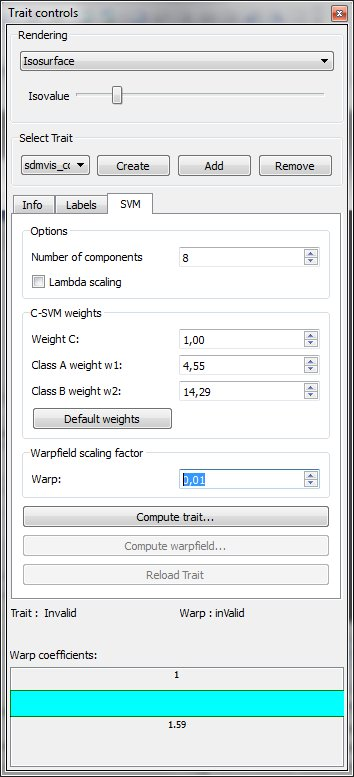
\includegraphics[width=0.2\textwidth]{screenshots/trait-ctrl-3}
\par\end{center}
\begin{itemize}
\item traits according to a specific grouping (also called labelling or
classification) can be loaded, created or deleted
\item create a trait:

\begin{itemize}
\item enter a unique identifying text (keep it short)
\item enter a description (optional and changeable later on; e.g. to make
some observation notes)
\item go to the second tab and enter the labelling (either manually or via
a textfile)
\item go to the third tab and adjust the SVM parameters (details TBD)
\item compute the trait
\item compute the trait warpfield
\end{itemize}
\end{itemize}

\subsection{Refine shape model according to Region of Interest}

\texttt{{[}Specify ROI{]}}

\noindent \begin{center}
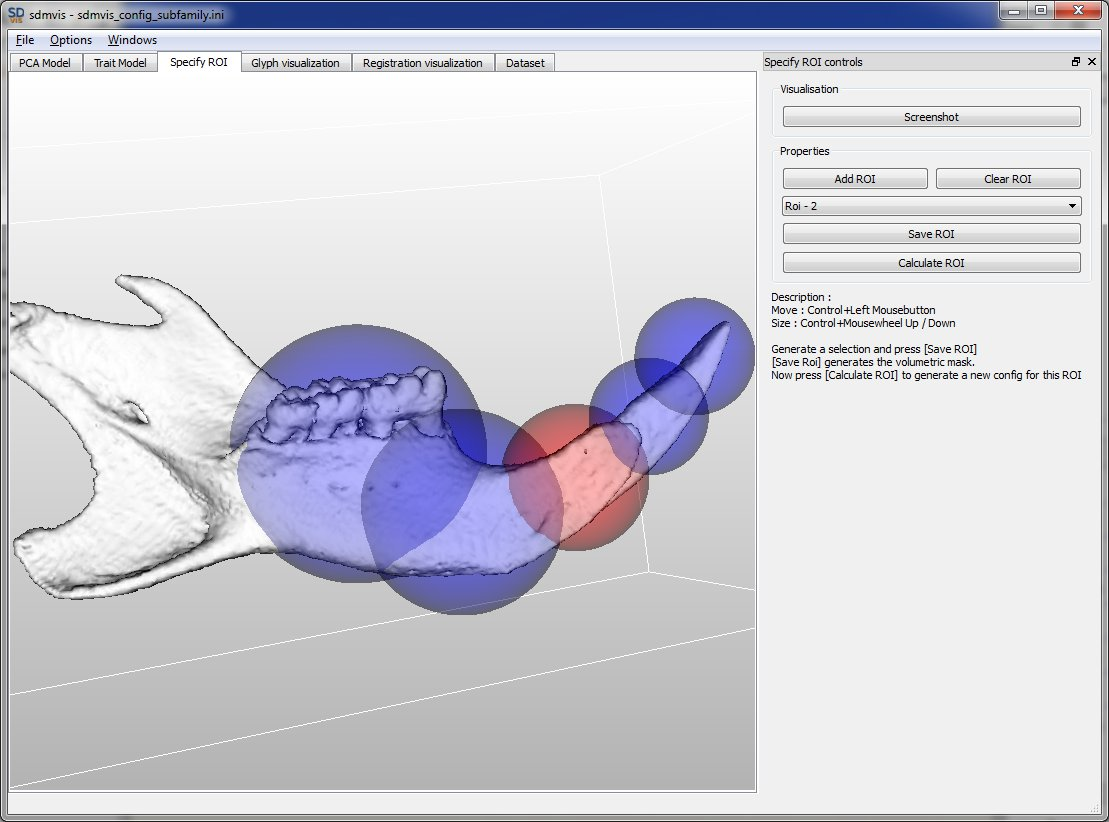
\includegraphics[height=6cm]{screenshots/sdmvis_roi}
\par\end{center}

TBD


\subsection{Subset Selection (not available yet)}


\subsection{Trait Quantification (not available yet)}
\end{document}
